\documentclass{article}
\usepackage{../fasy-hw}
\usepackage{ wasysym }
\usepackage{graphicx}

%% UPDATE these variables:
\renewcommand{\hwnum}{1}
\title{Discrete Structures, Homework 1}
\author{Patrick O'Connor (Patrick OConnor)}
\collab{n/a}
\date{due: 22 January 2021}

\begin{document}

\maketitle

This homework assignment should be
submitted as a single PDF file both to D2L and to Gradescope.

General homework expectations:
\begin{itemize}
    \item Homework should be typeset using LaTex.  (Note: if you are still
        having trouble with your setup, please reach out to the instructor and
        TA).
    \item Answers should be in complete sentences and proofread.
    \item You will not plagiarize.
    \item List collaborators at the start of each question using the
        \texttt{collab} command.
    \item Put your answers where the \texttt{todo} command currently is (and
        remove the \texttt{todo}, but not the word \texttt{Answer}).
\end{itemize}

% ============================================
% ============================================
\nextprob{Getting to Know Your Classmates}
\collab{n/a}
% ============================================
% ============================================

Find a different classmate for each of the following:
\begin{enumerate}
    \item Was born in the same month as you (year can be different).
        \paragraph{Answer}Shreya Deb - September

    \item Has a shared hobby with you.
        \paragraph{Answer}Fly fishing: Larson D Brandstetter

    \item Has the same middle initial as you.
        \paragraph{Answer}Using my one pass.

    \item Lives in a different building than you.
        \paragraph{Answer}Alex O van Dijken: He lives in North Hedges

    \item Has eaten at at least one restaurant or traveled to at least one city that you have not been
        (yet).
        \paragraph{Answer}Braeden J Hunt: San Diego

\end{enumerate}

% ============================================
% ============================================
\nextprob{Why Proofs?}
\collab{N/A}
% ============================================
% ============================================

Much of this class is spent learning how to prove things.  Explain why it is
important to you, as a computer scientist, to know how to prove things
mathematically.

\paragraph{Answer}As a computer scientist as opposed to a a software developer, 
proofs are extremely useful for ensuring that you have properly solved the problem at hand. 
The study of computer science compared to IT or hardware/electrical engingeer is focused more on solving problems with the tools of a computer. 
CS is fundamentally focused on the theory and practice of computation and can be practiced without a keyboard in your fingers. 
Although I stated that IT is different it is possible that similar problems such as memory management are essential for both. 
Overall these algorithms that are used to handle data or manage memory are based in logic and within the theoretical CS field using formal methods, 
complexity, and computability and using math to prove that this is proved is essential for making true statements.


% ============================================
% ============================================
\nextprob{A Proof}
\collab{N/A}
% ============================================
% ============================================

Prove that $6\Z \subset 2\Z$.

\paragraph{Answer}Let n $\in$ $6\Z$, By Definition of $6\Z$ we know that n is a multiple of 6. 
This can be explained as n = 9 * m where m is an integer. 
Then, n = 2(3 * m), therefore n = 2k where k = (3 * m), which means that n $\in$ $2\Z$ . 


% ============================================
% ============================================
\nextprob{Grace Hopper}
\collab{N/A}
% ============================================
% ============================================

Write a short (1-2 paragraph) biography of Grace Hopper.
\textbf{In your own words}, describe who they are and why they are important in
the history of computer science.  If you use external resources, please provide
proper citations.

\paragraph{Answer}Grace Murray Hopper was an American computer scientist and United States Navy rear admiral.
 While acheiving great rank in the United States Navy is one of her great life accomplishments; 
many of her great accomplishments were done in the academic world. 
Hopper started her academic career at the Ivy league school Yale and graduated with a degree in mathematics. 
Once graduated she continued her work in the mathematics department as a professor at Vassar College in New York.
 Around the same time as World War 2, Hopper joined the Navy Reserves as she was denied enlistment in the U.S. Navy. 
Roughly four years after joining the reserves, Hopper began her computing career on the Harvard Mark 1 team. 
Excelling at this job Hopper continued on the computing path and worked with Eckert-Mauchly Computer Corporation where 
she assisted in devoloping the UNIVAC 1 computer. The UNIVAC 1 was the first general purpose digital computer and 
could do relatively simple arithmetic and data transport operations.

Once the first digital computer was created, she focused on creating a linker that would convert english terms in machine code. 
Around 1952, Hopper finished her program linker and the first compiler was created. 
From their she branched into creating more computer languages and assisted in the creation of FLOW-MATIC and later COBOL. 
Unfortunely her private sector computer science career was put on hold when recalled to active duty for the Navy in 1967. 
During this time she reflected and wrote about her computing experiences during her time serving the US government. 
After serving for 9 years she retired from the forces and went back to the private sector to work as a consultant for Digital Equipment Corporation. 
During her time working as a consultant she represented the company at forums and served on various industry commitees until her death at age 85 in 1992.

\url{https://news.yale.edu/2017/02/10/grace-murray-hopper-1906-1992-legacy-innovation-and-service}
\url{https://www.britannica.com/biography/Grace-Hopper}


% ============================================
% ============================================
\nextprob{Bonus Question!}
\collab{N/A}
% ============================================
% ============================================

Use the `figure` environment to add a figure that provides the solution to
Exercises set 1.4, Problem 4.  Your figure can be hand drawn and scanned, or can
be made using a tool such as Inkscape.

\paragraph{See Figure}
\begin{figure}
  \caption{Edge 1 is connected to vertex 1. 
Edge two has endpoints on vertex 2 and vertex 3. 
Edge 3 has endpoints on vertex 2 and vertex 3. 
Edge 4 has endpoints on vertex 1 and vertex 5.}
  \centering
  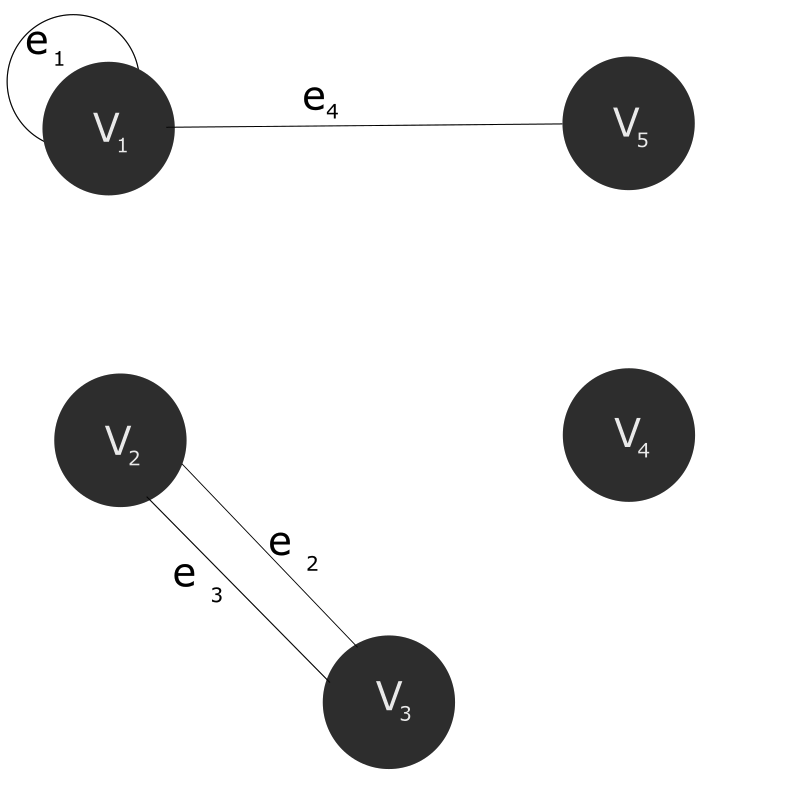
\includegraphics[width=0.5\textwidth]{ExcerciseProblem04}
  \label{fig:P04}
\end{figure}

Figure \ref{fig:P04} shows the figure.


\end{document}

